%Author: Brills(Brillsp@gmail.com)
%
%

\documentclass{beamer}
\usepackage{caption}
\usepackage{listings} %source code printing support
\lstset{ language={[ANSI]C},
         showspaces=false,
         showtabs=false,
         tabsize=4,
         frame=single,
         framerule=1pt,
         %numbers=left,
         %numberstyle=\small,
         basicstyle=\tt,
         directivestyle=\tt,
         identifierstyle=\tt,
         commentstyle=\tt,
         stringstyle=\tt,
         keywordstyle=\color{blue}\tt }
\mode<presentation>
{
%   \usetheme[blue,noshadow]{Trondheim}
%   \usetheme[blue,minimal]{Trondheim}
%  \usetheme[blue,compress,numbers,nonav]{Trondheim}
%\usetheme[sand,compress,numbers,nonav,innovation]{Trondheim}
%\usetheme[sand,compress,numbers,nonav]{Trondheim}
%\usetheme{Berlin}
%\usecolortheme{ntnuold}
%\usetheme{Singapore}
%\usetheme{Warsaw}
\usetheme{CambridgeUS}
\usefonttheme[onlymath]{serif}
\setbeamercovered{transparent}
}
\usepackage[absolute,overlay]{textpos}
\usepackage{fontspec}
\usepackage{graphicx}
\newfontfamily\zhfont[BoldFont=Microsoft YaHei]{SimSun} %设置中文
\newfontfamily\zhpunctfont{SimSun} % 设置中文
 
\setmainfont{Consolas}           %这里设置英文衬线字体
\setmonofont{Consolas}                     %英文等宽字体
\setsansfont{Consolas}               %英文无衬线字体
 
\usepackage{zhspacing}
\zhspacing
\title{MiniC编译器实习项目}
\author{彭焯\and 王衎 \and 华连盛 \and 李春奇}
\date{code.google.com/p/minic}
\institute{PKU}
\newcommand{\tabincell}[2]{\begin{tabular}{@{}#1@{}}#2\end{tabular}}
%表格内换行
\begin{document}

\AtBeginSection{                              % 在每个Section前都会加入的Frame

  \frame[allowframebreaks]{
  	\frametitle{摘要}
	\tableofcontents[current,currentsection]
  }
}
%\AtBeginSubsection[]                            % 在每个子段落之前
%{
%  \frame<handout:0>                             % handout:0 表示只在手稿中出现
%  {
%    \frametitle{框架}
%    \tableofcontents[current,currentsubsection] % 显示在目录中加亮的当前章节
%  }
%}
\begin{frame}
  \titlepage
\end{frame}
\frame[allowframebreaks]%
\begin{frame}
  \frametitle{摘要}
  \tableofcontents
\end{frame}


\section{项目概览}
\subsection{项目需求}
\begin{frame}
	\frametitle{项目需求}
	\noindent
	实现一个C语言子集(MiniC)的编译器,要求:
	\begin{itemize}
		\item 目标机器为Unicore32
		\item 输入MiniC源代码,生成Unicore32汇编代码。链接交由Unicore32二进制工具链完成
		\item 链接后的程序能在Unicore32实体机器上运行,且能够在同时设计的Unicore32模拟器上运行\footnote{体系实习项目}
		\item 实现包括指令调度在内的编译优化
		\item 通过对模拟器相关参数的修改,考察编译-ISA对性能的综合影响
	\end{itemize}
\end{frame}

\subsection{项目框架}
\begin{frame}
	\frametitle{项目框架}
	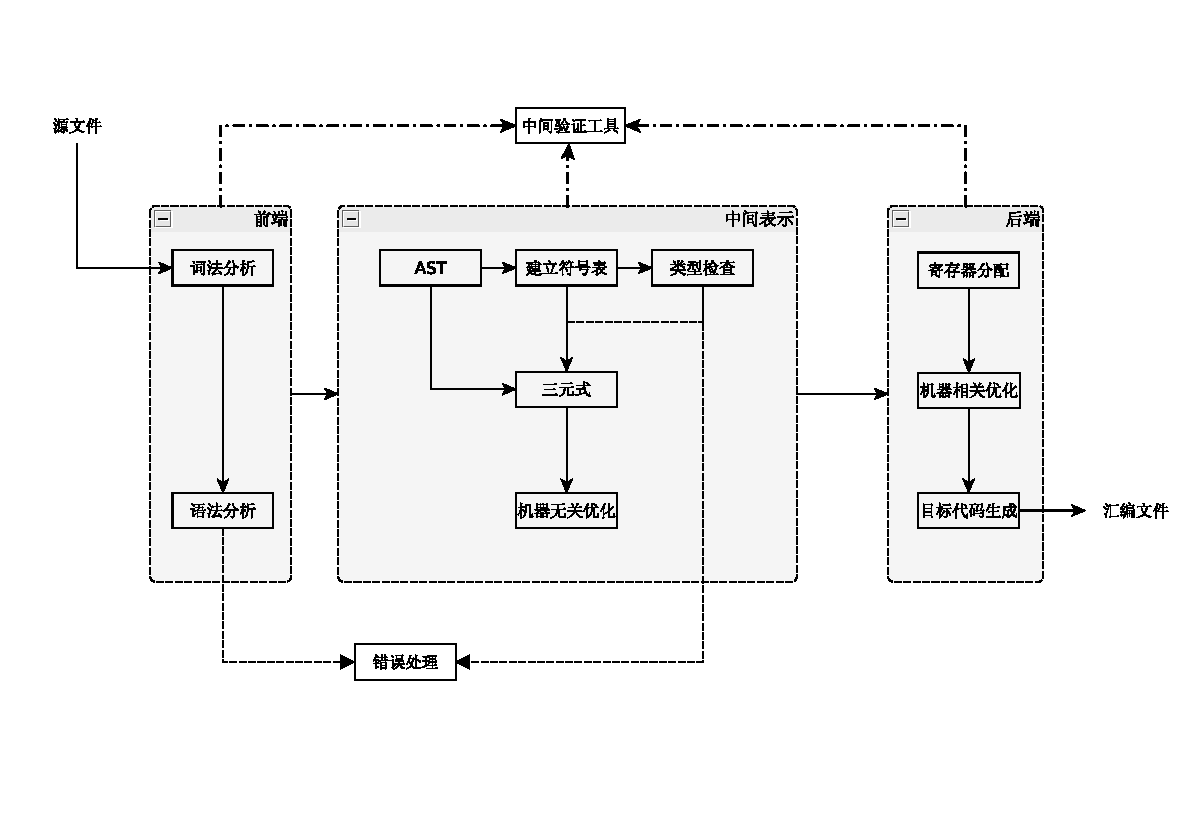
\includegraphics[scale=0.5]{main_structure.eps}
\end{frame}

\section{前端}
\begin{frame}
	\frametitle{前端}
	\begin{block}{\phantom{x}}
	\begin{itemize}
		\item 词法分析使用flex辅助完成
		\item 语法分析使用bison辅助完成,生成AST
		\item 简单的预处理器,支持注释
		\item 简单的错误提示功能(见下图)
	\end{itemize}
	\end{block}
	\begin{block}{错误提示}
	\begin{columns}
		\column{0.3\textwidth}
		\begin{flushleft}
		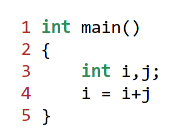
\includegraphics[scale=0.5]{error_example_left.png}
		\end{flushleft}
		\column{0.5\textwidth}
		\begin{flushleft}
		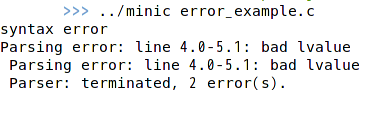
\includegraphics[scale=0.5]{error_example_right.png}
		\end{flushleft}
	\end{columns}
	\end{block}
\end{frame}

\section{中间表示}
\subsection{AST}
\begin{frame}
\frametitle{抽象语法树AST}
\noindent
AST是MiniC的第一重中间表示,符号表生成和类型检查检查在AST上进行。
\begin{columns}
	\column{0.4\textwidth}
	\begin{flushleft}
	\phantom{x}
	\vspace{0.2cm}
	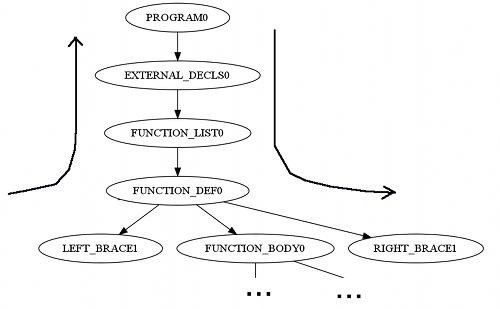
\includegraphics[scale=0.4]{AST_travel.png}
	\end{flushleft}
	\column{0.4\textwidth}
	\small{我们设计了通用的AST遍历模板,只需要在其上填入所需的操作(函数)就能够完成符号表生成/类型检查}
\end{columns}
\end{frame}

\subsection{符号表}
\begin{frame}
\frametitle{符号表}
\noindent
为了支持支持复合语句中的声明,符号表采用树状组织,具体实现采用可扩张线性表。
\begin{columns}
	\column{0.4\textwidth}
	\begin{center}
	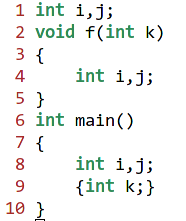
\includegraphics[scale=0.45]{symtbl_example.png}
	\end{center}
	\column{0.4\textwidth}
	\begin{center}
	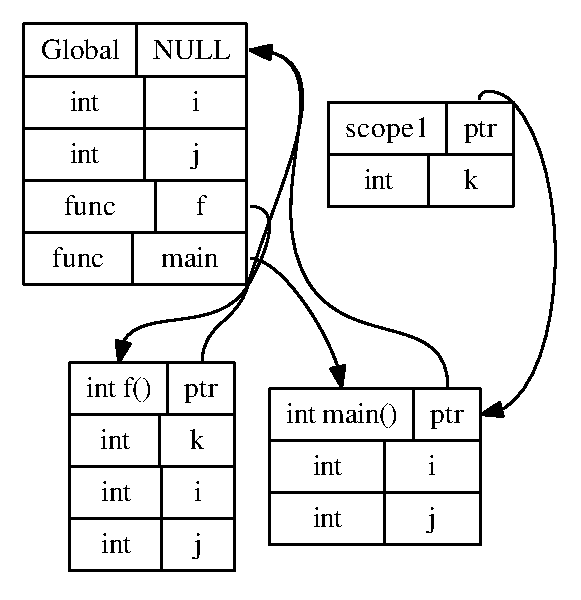
\includegraphics[scale=0.4]{symtbl.eps}
	\end{center}
\end{columns}
\end{frame}

\subsection{类型检查}
\begin{frame}
	\frametitle{类型检查}
\noindent
	类型检查负责报告:
	\begin{itemize}
		\item 使用未声明的变量;调用未声明的函数
		\item 函数调用传参个数不符
		\item 函数调用传参类型不匹配(警告或错误)
		\item 函数返回值同表达式中算符/操作数类型不匹配(警告或错误)
		\item 非法的指针运算,如相加、相乘和不同类型指针相减
		\item 不同存储类型的变量运算,如\lstinline|char|和\lstinline|int|相加(警告)
	\end{itemize}
\end{frame}
\subsection{三元式}
\begin{frame}
	\frametitle{三元式}
	\noindent
	三元式是MiniC的第二重中间表示,它由AST经过变换而来,在表达能力上同源语言等价。机器无关的优化、目标代码生成均以它为基础进行,下表是三元式指令及功能。

除了运算指令和条件跳转、无条件跳转指令外,三元式中有如下的特殊指令:
\begin{center}
	\begin{tabular}{|l|l|l|l|}
	\hline
		指令类型 & 举例 & 作用 \\
		\hline
		比较指令 & less  & 关系成立值为1,否则0 \\
		\hline
		rb操作指令 & setrb, getrb & 设置或读取rb的值 \\
		\hline
		函数调用指令 & param, call& 传参,函数调用\\
		\hline
		常量表示指令 & Imm, c\_str & 表示一个常量或字符串\\
	\hline
	\end{tabular}
\end{center}
\end{frame}
\begin{frame}
	\frametitle{三元式(续):布尔表达式的翻译}
	下面主要介绍布尔表达式的翻译:
	\begin{columns}
		\column{.6\textwidth}
			由于三元式中同一个临时变量不能有两次赋值,我们假设有一个rb寄存器,并且用setrb和getrb来实现给同一临时变量赋值。

右图是k=(a||b)\&\&i的基本块。
\alert{在目标代码生成时,我们没有采取直接翻译的方式处理setrb和getrb.}
		\column{.3\textwidth}
			\begin{center}
			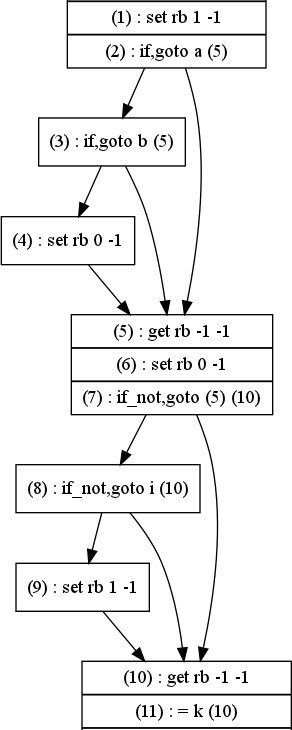
\includegraphics[scale=0.24]{bool_triple_example.png}
			\end{center}
	\end{columns}
\end{frame}

\section{后端}
\subsection{目标机器寄存器使用规范}
\begin{frame}
\frametitle{目标机器寄存器使用规范}
\begin{center}
	\begin{tabular}{|l|l|l|}
	\hline
		寄存器 & Unicore32 & MiniC \\
	\hline
		r0-r3 & 传递参数和返回值& \alert{\tabincell{l}{传递参数和返回值;在函数内\\用于无寄存器变量的装入和运算}} \\
	\hline
		r4-r15 & caller save & caller save$^*$\\
	\hline
		r17-r25 & callee save & callee save$^*$\\
	\hline
		r26 & 静态基址 & \alert{用于读取大立即数地址}\\
	\hline
		r27 & 栈帧基址 & 栈帧基址\\
	\hline  
		r28 & 调用者SP & \alert{传参时用于装入和运算;生成立即数}\\
	\hline 
		r29 & 栈基址 & 栈基址 \\
	\hline
		r30 & 返回地址 & 返回地址 \\
	\hline 
		r31 & PC & PC \\
	\hline
	\end{tabular}
\end{center}
\emph{* 数目可调}
\end{frame}

\subsection{栈帧及全局区}
\begin{frame}
	\frametitle{栈帧及全局区}
	\begin{columns}
		\column{0.4\textwidth}
			\begin{itemize}
				\item 栈帧布局和数组存放规则见右图
				\item 无法使用立即数寻址的大立即数保存在代码段,使用PC相对寻址得到
				\item 全局变量、字符串常量保存在全局区,并将其指针放在代码段
				\end{itemize}
		\column{0.65\textwidth}
		\begin{columns}
			\column{0.32\textwidth}
			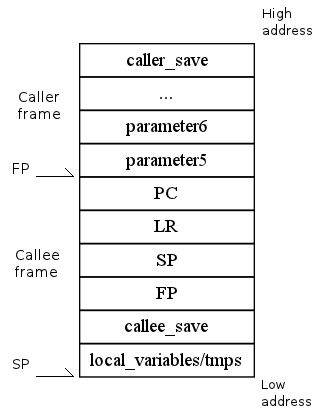
\includegraphics[scale=0.3]{stack_frame.png}
			\column{0.3\textwidth}
			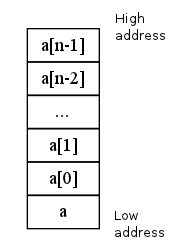
\includegraphics[scale=0.3]{local_array.png}
		\end{columns}
	\end{columns}
\end{frame}
\subsection{寄存器分配}
\begin{frame}
	\frametitle{寄存器分配}
	\begin{columns}
	\column{0.4\textwidth}
	\begin{itemize}
		\item 依赖于活跃变量分析
		\item 采用图染色法
		\item 小的删点策略改进,见右例
	\end{itemize}
	\column{0.65\textwidth}
	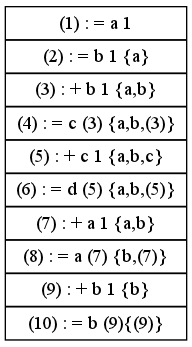
\includegraphics[scale=0.3]{register_allocation_triple.png}
	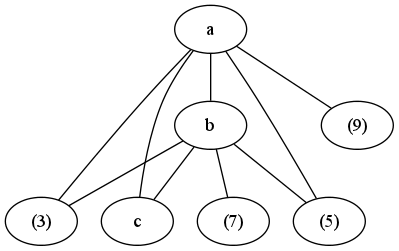
\includegraphics[scale=0.3]{interference_graph.png}
	\end{columns}
\end{frame}
\subsection{寄存器保护-推栈策略}
\begin{frame}
%TODO:registers push/pop
	\frametitle{寄存器保护-推栈策略}
	\begin{itemize}
		\item 局部变量
		\item 临时变量
		\item 全局变量
	\end{itemize}
\end{frame}
\subsection{setrb/getrb的处理}
\begin{frame}
\frametitle{setrb/getrb的处理}
\begin{center}
\includegraphics[scale=0.5]{setrb.png}
\end{center}
\end{frame}

\section{编译优化}
\subsection{数据流分析}
\begin{frame}
	\frametitle{数据流分析}
	\noindent
	\begin{itemize}
		\item 在三元式上进行数据流分析
		\item 设计了适用于迭代算法的通用的数据结构
		\item 进行了如下分析:
		\begin{itemize}
			\item 活跃变量分析
			\item \alert{可用表达式传播}
			\item \alert{指针分析}
		\end{itemize}
	\end{itemize}
\end{frame}
\begin{frame}
	\frametitle{可用表达式传播}
	\begin{columns}
		\column{0.5\textwidth}
		\begin{itemize}
			\item 依赖于可用表达式分析
			\item 如果某三元式计算的表达式可用且所有可用表达式交汇于一点,则用该点替换下面所有用到该三元式标号的三元式,并删除该表达式。
			\item 迭代进行,直到没有三元式被删除
			\item \alert{类似于,但性能劣于复写传播}
		\end{itemize}
		\column{0.6\textwidth}
		\begin{columns}
			\column{0.3\textwidth}
			\includegraphics[scale=0.26]{before_available_expr.jpeg}
			\column{0.3\textwidth}
			\includegraphics[scale=0.26]{after_available_expr.jpeg}
		\end{columns}
	\end{columns}
\end{frame}
\begin{frame}
	\frametitle{指针分析}
		\begin{itemize}
			\item 用于解决指针操作时寄存器-栈帧同步的问题
			\item 算法最终能得到在每个程序点,每个指针的指向状态。可以根据该状态比较精确地进行同步
			\item 基于数据流分析:
			\begin{itemize}
				\item 对象:序对$(p,v)$,代表指针$p$指向$v$
				\item $GEN(B)$基本块$B$中产生的序对集合
				\item $KILL(B)$基本块$B$中注销的序对集合
				\item 迭代方向:正向
				\item 迭代方程:$OUT(N) = GEN(N)+(IN(N)-KILL(N))$ $IN(N)=\bigcup_{P\in predecessor(N)}OUT(P)$
			\end{itemize}
		\end{itemize}
\end{frame}
\begin{frame}
	\frametitle{指针分析(续)——性能}
	\begin{columns}
		\column{0.6\textwidth}
		\noindent
		对于右图的例子,下面三种方法在第9行、第12行、第14行需要的同步次数如下:
		\begin{itemize}
			\item 每次同步所有变量:3次;3次;3次
			\item 扫描一次记录每个指针指过的所有变量: \alert{2次};3次;3次
			\item 利用指针分析的结果: \alert{2次};3次;\alert{1次}			
		\end{itemize}
		\column{0.4\textwidth}
		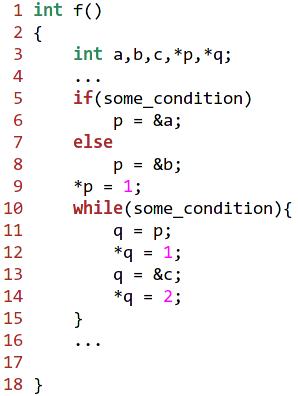
\includegraphics[scale=0.33]{pointer_analysis_example.png}
	\end{columns}
\end{frame}
\subsection{中间代码上的窥孔优化}
\begin{frame}
	\frametitle{中间代码上的窥孔优化}
%	\begin{block}{\phantom{x}}
	\begin{itemize}
		\item 常量表达式计算:计算出两个操作数都是立即数的三元式的值,如果用到该三元式值的三元式又能够直接计算,那么迭代地进行这个过程,直到结果是编译时不可计算的为止。(不考虑对于带有常数的布尔运算。)
		\item 简单的强度削减:乘以2的幂次改为左移(乘法2 cycle而左移1 cycle)
	\end{itemize}
	\begin{columns}
		\column{0.3\textwidth}
		\begin{flushright}
			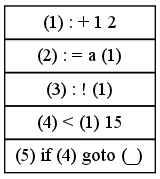
\includegraphics[scale=0.3]{before_const_expr.png}
		\end{flushright}
		\column{0.3\textwidth}
		\begin{flushleft}
			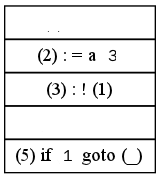
\includegraphics[scale=0.3]{after_const_expr.png}
		\end{flushleft}
	\end{columns}
\end{frame}

\subsection{目标代码上的窥孔优化}
\begin{frame}
	\frametitle{合并地址计算和访存语句}
	\begin{itemize}
		\item 目标代码由三元式翻译而来,不能直接利用Unicore32的寄存器位移读取/写入指令
		\item 发现计算地址和访存指令,将它们合并
	\end{itemize}
	下例是\lstinline|a[i] = 1|的三元式、优化前汇编码和优化后汇编码
	\begin{columns}
		\column{0.4\textwidth}
		\begin{center}
			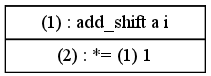
\includegraphics[scale=0.4]{ldst_peephole_triple.png}
		\end{center}
		\column{0.6\textwidth}
			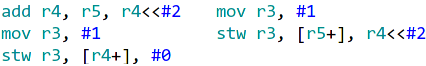
\includegraphics[scale=0.4]{ldst_peephole_example.png}
	\end{columns}
\end{frame}

\begin{frame}
	\frametitle{删除冗余的mov}
	\begin{itemize}
		\item 由于三元式直接翻译到Unicore32汇编不能很好的利用三个操作数的汇编指令,会产生出很多冗余的\lstinline|mov|
		\item 我们做了窥孔优化来找到符合以下条件的\lstinline|mov|,删除它,并修改其后用到它的目标寄存器的语句的源寄存器:
		\begin{itemize}
			\item 从\lstinline|mov|指令的源寄存器最近的一次定值开始,到\lstinline|mov|指令之间没有对\lstinline|mov|的目标寄存器引用。
			\item 从\lstinline|mov|指令开始,将\lstinline|mov|指令的源寄存器替换为目标寄存器时不会产生冲突。
		\end{itemize}
	\end{itemize}
	
	\begin{center}
	\includegraphics[scale=0.5]{redundent_mov_remove.png}
	
	\end{center}
\end{frame}
\subsection{尾递归优化}
\begin{frame}
	\frametitle{尾递归优化}
	尾递归优化能将符合如下条件的函数调用转换为迭代(即\alert{免去保存和回复现场、建立栈帧等操作}):
	\begin{enumerate}
		\item 递归调用
		\item 该调用语句是本函数除返回语句以外的最后一条语句
		\item 该函数没有返回值
	\end{enumerate}
\end{frame}
\begin{frame}
	\frametitle{尾递归优化-续:一个例子}
	%下面是一个快速排序的程序片段,以及优化前、优化后的汇编代码:
	\begin{columns}
		\column{0.3\textwidth}
		\begin{flushleft}
		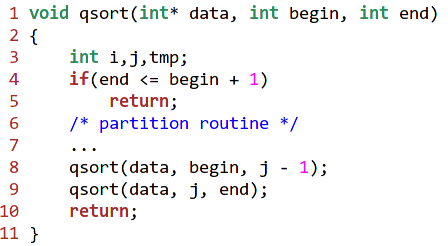
\includegraphics[scale=0.3]{tail_recursion_example.png}
		\end{flushleft}
		\column{0.7\textwidth}
		\begin{center}
		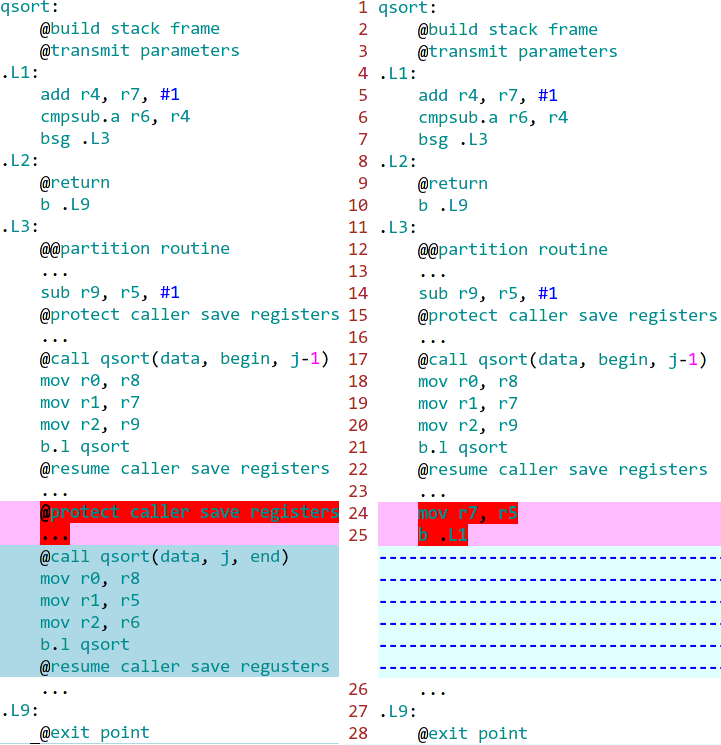
\includegraphics[scale=0.2]{tail_recursion.png}
		\end{center}
	\end{columns}
\end{frame}
\subsection{指令调度}
\begin{frame}
	\frametitle{指令调度}
	根据Unicore32指令系统体系结构,只有载入指令和运算指令可能产生的数据相关无法转发,需要等待一个cycle。指令调度的目的就是尽量让这种数据相关不发生。
	
	算法作用范围是目标代码上的基本块,基于一个“数据依赖图”:若指令\lstinline|i|的源操作数依赖于指令\lstinline|j|的执行结果,则建立\lstinline|j|到\lstinline|i|的一条边;算法的思想是先按顺序对\lstinline|ldw|执行一种带优先级的拓扑排序:遇到\lstinline|ldw|则安排执行所有它依赖的指令(包括反依赖关系),然后从未安排执行过的指令中,取一条入度为0的指令,要求它尽量不依赖于\lstinline|ldw|的结果,排在\lstinline|ldw|之后;最后对还未被安排的非\lstinline|ldw|指令再进行一次拓扑排序即可。
\begin{columns}
	\column{0.2\textwidth}
		\includegraphics[scale=0.4]{before_assemble_dispatch.png}
	\column{0.4\textwidth}
		\includegraphics[scale=0.3]{assemble_rely_graph.png}
	\column{0.3\textwidth}
		\includegraphics[scale=0.4]{after_assemble_dispatch.png}
\end{columns}
\end{frame}

\begin{frame}
	\begin{center}
	\Large{演示与Q\&A}
	\end{center}
\end{frame}
\end{document}
